\documentclass[12pt,journal,compsoc]{IEEEtran}

\newcommand{\subparagraph}{}

\usepackage[compact]{titlesec}
\titlespacing{\section}{0pt}{1ex}{1ex}
\titlespacing{\subsection}{0pt}{1ex}{0.5ex}
\titlespacing{\subsubsection}{0pt}{0.5ex}{0ex}

\usepackage{graphicx}
\graphicspath{ {../src/img/} }
 
\begin{document}
%
% paper title
% can use linebreaks \\ within to get better formatting as desired
% Do not put math or special symbols in the title.
\title{Assignment 2}

\author{Shubham~Singla,
        Harsh~Kumar and~
        Rupesh~Kashyap}% <-this % stops a space


% make the title area
\maketitle

\section{Introduction}
\IEEEPARstart{F}{ollowing} report contains observation for the $4$ data sets provided in the assignment namely, FMNIST, Medical data, Railway data and River Data set. The observations contain the performance of different machine learning algorithms on the above mentioned data sets. The algorithms implemented are PCA, Linear regression with polynomial of different degrees phi functions, logitic regression using softmax, FLDA, PCA and SVM for multi class cases. Results have been summarized below in the form of accuracy, precision, recall, f-score, micro and macro average precision, recall and f-score.

\section{Medical Data}
\noindent Each of 'Healthy', 'Surgery' and 'Medication' are assigned a number $0$, $1$ and $2$ respectively. Thus, it reduces to a problem of having labeled data with $3$ classes and $3$ features for each data point. The data was observed in 3D and 2D using PCA. Standardization of data followed by a 75/25 split into train and dev set was done. Perceptron, FLDA, SVM (with RBF, Linear, Polynomial and sigmoid kernel) and Logistic Regression (involving softmax activation) were applied. Perceptron and FLDA used a similar approach as of softmax for classification.
\begin{center}
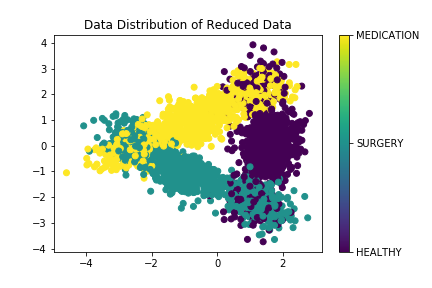
\includegraphics[scale=0.35]{2d_medical.png}

{\small Fig. 1 Visualization of Data in 2D}
\end{center}

\begin{center}
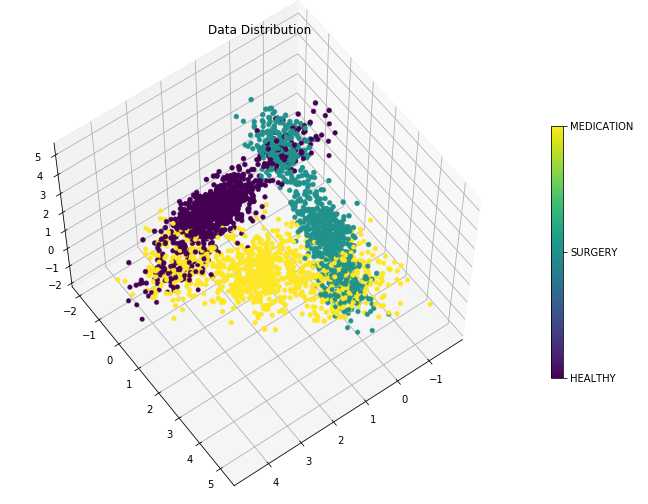
\includegraphics[scale=0.35]{3d_medical.png}

{\small Fig. 2 Visualization of Data in 3D}
\end{center}

\subsection{Observations}
\subsubsection{Perceptron Model}
\begin{center}
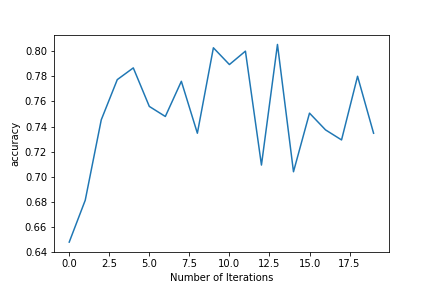
\includegraphics[scale=0.35]{perceptron_accuracy.png}

{\small Fig. 3 Variation of Accuracy on Y-axis Vs Number of iterations*500 + 100 on X-axis}
\end{center}

Perceptron model gave best accuracy after $6600$ iterations.
Performance on test data-\\ 
Accuracy - $0.8053$\\ F-Score (Class 1) - $0.8523$\\
F-Score (Class 2) - $0.8371$\\ F-Score (Class 3) - $0.7$\\ Macro Average F-Score - $0.8108$\\
Micro Average F-Score - $0.8053$\\

\subsubsection{FLDA Model}
\noindent Fisher Linear Discriminant Analysis gave the following results -
Performance on test data-\\ 
Accuracy - $0.811$\\ F-Score (Class 1) - $0.8738$\\
F-Score (Class 2) - $0.7894$\\ F-Score (Class 3) - $0.7728$\\ Macro Average F-Score - $0.8139$\\
Micro Average F-Score - $0.811$\\

\subsubsection{Logit Model (Softmax Function)}
\begin{center}
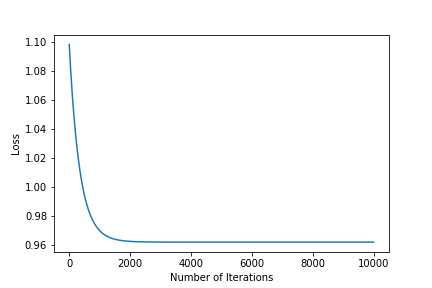
\includegraphics[scale=0.35]{softmaxloss.png}

{\small Fig. 3 Variation of Loss Vs Number of iterations}
\end{center}

Loss in logit model stopped decreasing after $2000$ iterations.
Performance on test data-\\ 
Accuracy - $0.8053$\\ F-Score (Class 1) - $0.8523$\\
F-Score (Class 2) - $0.8371$\\ F-Score (Class 3) - $0.7$\\ Macro Average F-Score - $0.8108$\\
Micro Average F-Score - $0.8053$\\

\subsubsection{SVM Model}
\begin{center}
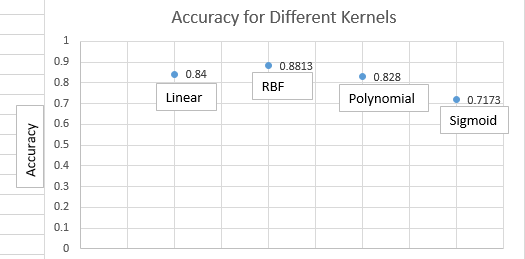
\includegraphics[scale=0.6]{svm_medical.png}

{\small Fig. 3 Comparing Accuracy on Y-axis Vs Different kernels used on X-axis}
\end{center}

Support Vector Machines gave best accuracy with rbf kernel.
Performance on test data-\\ 
\\
\noindent{
\begin{tabular}{|c|c|c|c|c|}
\multicolumn{5}{c}{SVM Classifier}\\
\hline
Kernel & Accuracy & F(C1) & F(C2) &  F(C3)\\
\hline
Linear &$0.84$ &$0.9018$ &$0.8366$ &$0.7848$ \\
\hline
RBF &$0.8813$ &$0.9127$ &$0.8893$ &$0.8405$ \\
\hline
Poly &$0.828$ &$0.8447$ &$.8288$ &$0.8139$ \\
\hline
Sigmoid &$0.7173$ &$0.7504$ &$0.7284$ &$0.6667$ \\
\hline
\end{tabular}
\newline
}

\subsection{Conclusion}
\noindent Maximum accuracy of $0.88$ for SVM classifier with rbf kernel is obtained. For logit model, loss decreased with the number of iterations and it stopped decreasing after a certain number of iterations. Perceptron model didn't converge meaning that the data is not linearly separable. Accuracy for perceptron model increased to a certain number of iterations after which it starts fluctuating. Maximum accuracy was obtained at around $6600$ iterations. It was also observed that on applying PCA and reducing the data to 2 dimensions resulted in decrease in the accuracy. 

\section{River Data}
\noindent River data contains a lot of noise as is clear from the image. It seems quite plausible that it won't be able to fit using linear model. Polynomial features were also tried and the results are tabulated below in the form of r-squared values.

\begin{center}
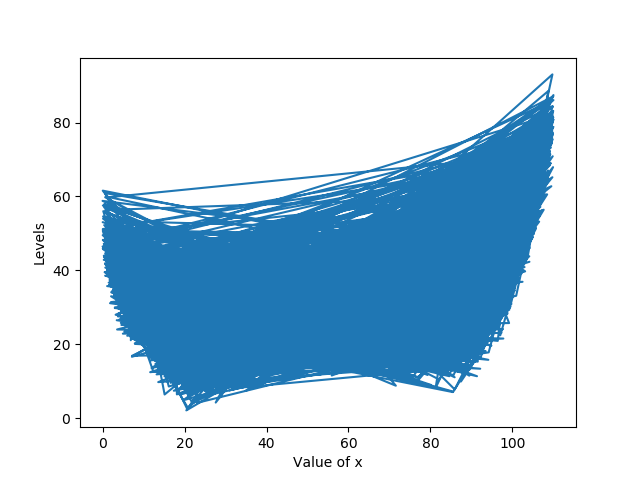
\includegraphics[scale=0.35]{River_dataset.png}

{\small Fig. 6 Visualizing River levels with x}
\end{center}

\begin{center}
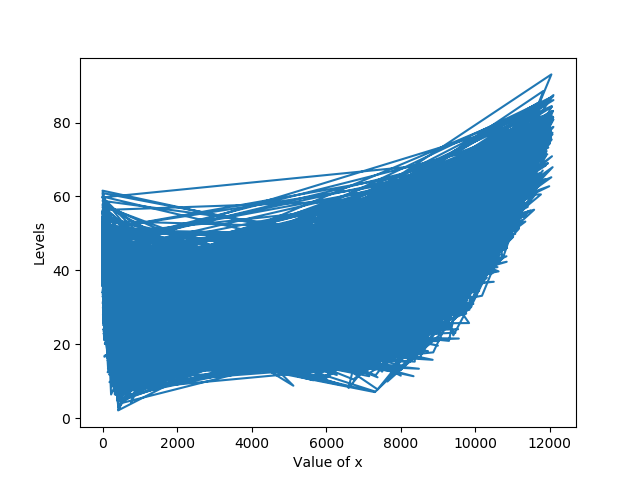
\includegraphics[scale=0.35]{River_dataset_squared.png}

{\small Fig. 7 Visualizing River levels with squared of x}
\end{center}

\subsection{Observations}

\begin{center}
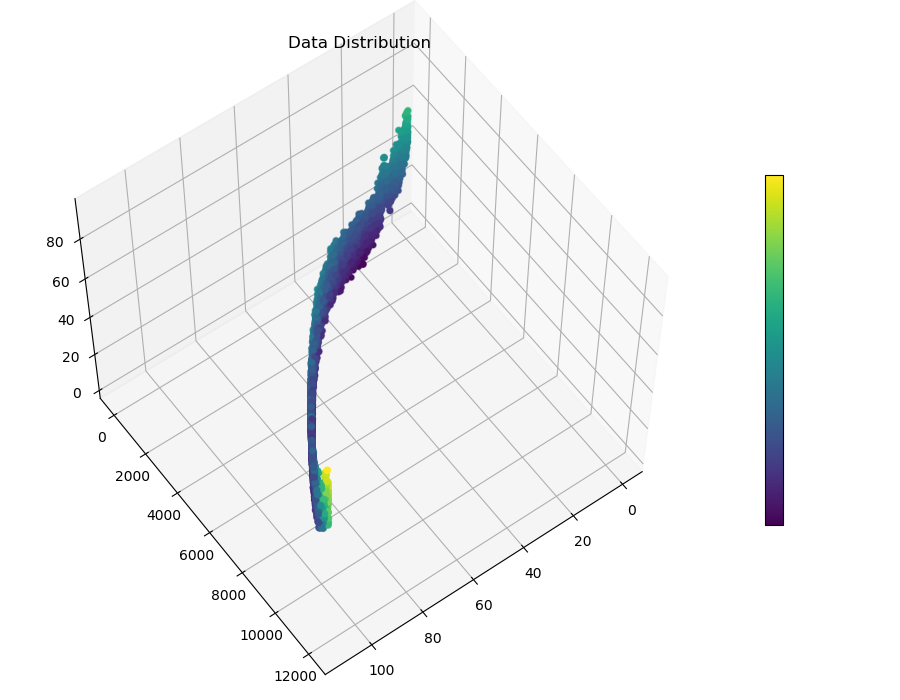
\includegraphics[scale=0.35]{3D.png}

{\small Fig. 7 Visualizing River levels with x and x-squared}
\end{center}

\noindent{
\begin{tabular}{|c|c|}
\multicolumn{2}{c}{Linear Regression}\\
\hline
Degree of Polynomial & R-squared\\
\hline
One &$0.126$\\
\hline
Two &$0.456$\\
\hline
Three &$0.498$\\
\hline
Four &$0.823$\\
\hline
Five &$0.823$\\
\hline
\end{tabular}
\newline
}
\\
\noindent \textbf{Maximum R-squared} is obtained for polynomial of \textbf{degree 4 - 0.823}.\\

\subsection{Conclusion}
We observed that value of R-squared became constant with increasing degree of polynomial. Also, we tried fitting exponential, square root and log after clipping minimum value to zero, results were more or less same.


\section{Railway Data}
\noindent The labels corresponding to each data point were in binary format denoting BOARDED AND NON-BOARDED CASES. This dataset is example of categorical data and discrete. The columns of SEX of passenger and TYPE OF COACH booked is converted into binaries using ONE-HOT encoding. Later models FLDA, perceptron, Logistic regression and SVM models are tested on standardised and non-standardised data.  

\begin{enumerate}
\item Using PCA to visualize the data in 2 dimensions.
\begin{center}
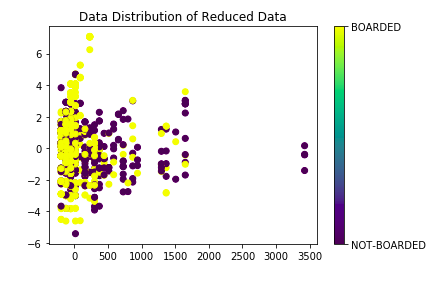
\includegraphics[scale=0.50]{report/2d_data.png}
{\small 
Fig. 1 Visualizing railway data in 2D using PCA}
\end{center}
\item Visualizing the class counts as this kind of data is usually skewed and this may affect the performance of classifiers.

\begin{center}
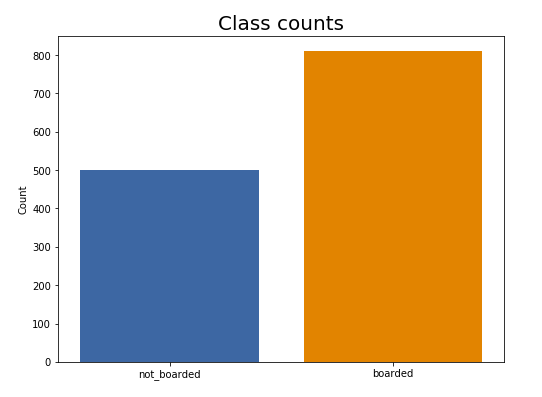
\includegraphics[scale=0.40]{report/classcounts.png}
{\small 
Fig. 2 Class counts of railway data}
\end{center}
\end{enumerate}
\subsection{Observations}
\subsubsection{Perceptron Model}
\begin{center}
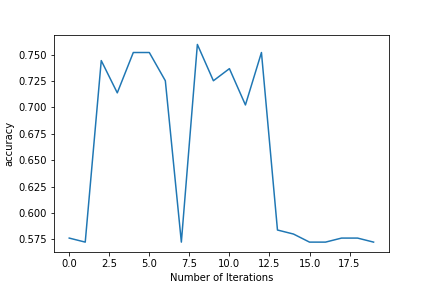
\includegraphics[scale=0.50]{report/perceptron_accuracy_harsh.png}

{\small Fig. 3 Variation of Accuracy on Y-axis Vs Number of iterations*500 + 100 on X-axis}
\end{center}

Perceptron model gave best accuracy around $4100$ iterations with non-standardized data.\\
Performance on data-\\ 
Training set accuracy: $0.7948$\\
Training set f1 score: $0.8456$\\
Test set accuracy: $0.7595$\\
Test set f1 score: $0.8141$\\
\begin{center}
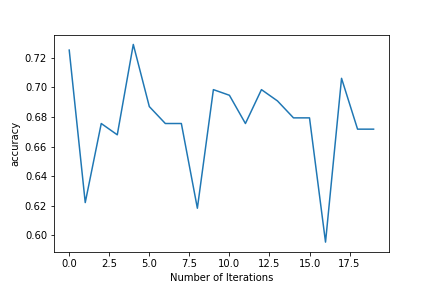
\includegraphics[scale=0.50]{report/scaled_perceptron.png}

{\small Fig. 4 Accuracy Vs Number of iterations*500 + 100 on scaled features}
\end{center}
Best accuracy on non scaled dataset is more than scaled which is very interesting.\\
Scaled dataset max accuracy around $2100$ iterations:$0.7290$ \\

\subsubsection{FLDA Model}
\noindent Fisher Linear Discriminant Analysis failed miserably on the binary featured dataset with Test set accuracy: $0.4427$
Test set f1 score: $0.0519$. But the performance was reasonable on scaled dataset.\\
Performance on scaled data-\\ 
Training set accuracy: $0.7299$\\
Training set f1 score: $0.7631$\\
Test set accuracy: $0.7748$\\
Test set f1 score: $0.7915$\\
\subsubsection{Logistic Regression(Sigmoid wrapping)}
\noindent This problem is binary classification, so the defined approach is using sigmoid as the wrapping function. The results using the softmax approach are also listed. On binary features, the sigmoid regression gave poor performance.

Training set accuracy: $0.629$\\
Training set f1 score: $0.772$\\
Test set accuracy: $0.572$\\
Test set f1 score: $0.728$\\
On scaled data:\\
Training set accuracy: $0.7929$\\
Training set f1 score: $0.8403$\\
Test set accuracy: $0.7862$\\
Test set f1 score: $0.8271$\\
\begin{center}
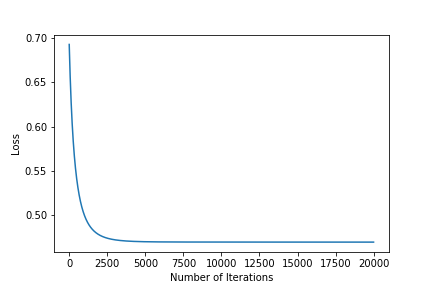
\includegraphics[scale=0.50]{report/logistic_loss20000.png}
{\small Fig. 5 Loss Vs Number of iterations; alpha=0.005; lambda=0.5}
\end{center}
\subsubsection{SVM Model}
\noindent SVM model was tested on the data using different kernels. Only the linear and the Guassian kernel could function on the non-standardized dataset. The results listed are obtained from the standardized dataset.

\begin{center}
    

SVM: \\  
\vspace{0.06cm} 
\begin{tabular}{|l|l|l|}
\hline
Kernel                                                           & Accuracy & F1-score \\ \hline
Linear                                                           & 0.7595    & 0.8012      \\ \hline
\begin{tabular}[c]{@{}l@{}}Gaussian \end{tabular} & 0.7633   & 0.8165
\\ \hline
\begin{tabular}[c]{@{}l@{}}Polynomial\end{tabular} & 0.7633   & 0.8176    \\ \hline
\begin{tabular}[c]{@{}l@{}}sigmoid\end{tabular} & 0.6793     & 0.7358       \\ \hline
\end{tabular}

\end{center}

\vspace{0.04cm} 
\subsection{Conclusion}
\noindent The discrete and categorical features of this dataset give rise to interesting behaviours. Standardizing the data to zero mean and unit variance improved the performance of FLDA, Logistic regression and SVM models significantly whereas the Perceptron model performed better on binary featured data(Test set accuracy:0.75). All the models performed in the range 0.70-0.80. The best model was obtained using Logistic regression on the scaled dataset achieving accuracy around 0.79 compared to SVM's 0.7633. Not many models give satisfactory results on discrete features except perceptron and SVM. The Perceptron algo does not converge. It fluctuates in regular intervals showing the non-separable nature of the data as can be seen in Fig. 3 and Fig. 4. 


\section{FASHION MNIST Data}

\noindent This is a multi-class classification problem where the feature vectors are sparse. Constrained by the memory and computational power, the number of experiments for this data set were reduced. Standardizing the data set with each feature having zero mean and unit variance resulted in unsatisfactory results. Therefore, another normalization technique was used where each example was scaled to have unit norm. Multi class discrimnative models: Perceptron, Logistic, FLDA , SVM were implemented. Here, assume number of components after PCA to be 80 unless stated.  

\subsection{Observations}

\subsubsection{Learning Algorithms}
\noindent{
\begin{center}
\noindent{
\begin{tabular}{|c|c|c|c|c|}
\multicolumn{4}{c}{FLDA}\\
\hline
Dim. & Acc. & Macro Avg. & Micro Avg.\\
\hline
$20$ &$0.713$ &$0.7223$ &$0.713$\\
\hline
$40$ &$ 0.7568$ &$0.7623$ &$0.7568$\\
\hline
$60$ &$0.7747$ &$0.7755$ &$0.7747$\\
\hline
$80$ &$0.7815$ &$0.7824$ &$0.7815$\\
\hline
$100$ &$ 0.784$ &$0.7852$ &$0.7847$\\
\hline
$200$ &$ 0.7934$ &$0.7939$ &$0.7934$\\
\hline
$300$ &$ 0.7978$ &$0.7972$ &$0.7978$\\
\hline
\end{tabular}
}
\end{center}
\begin{center}
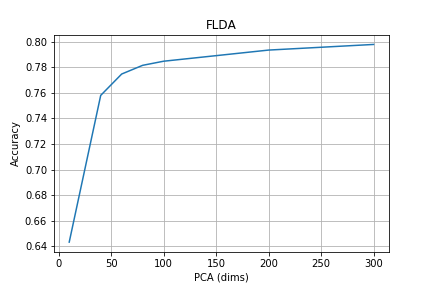
\includegraphics[height = 5cm, width= 7cm]{report/FLDA.png}
\end{center}
}

\begin{tabular}{|c|c|c|c|}
\multicolumn{4}{c}{Perceptron}\\ \hline
Dims & Acc.   & Macro Avg. & Micro Avg. \\ \hline
20   & 0.5967 & 0.5848  & 0.5967  \\ \hline
40   & 0.6971 & 0.6962  & 0.6971  \\ \hline
60   & 0.7224 & 0.7158  & 0.7224  \\ \hline
80   & 0.7173 & 0.7098  & 0.7173  \\ \hline
100  & 0.7219 & 0.7167  & 0.7219  \\ \hline
200  & 0.7263 & 0.7171  & 0.7263  \\ \hline
400  & 0.6998 & 0.7099  & 0.6998  \\ \hline
784  & 0.7981 & 0.8101  & 0.7981  \\ \hline
\end{tabular}

\newpage
\begin{center}
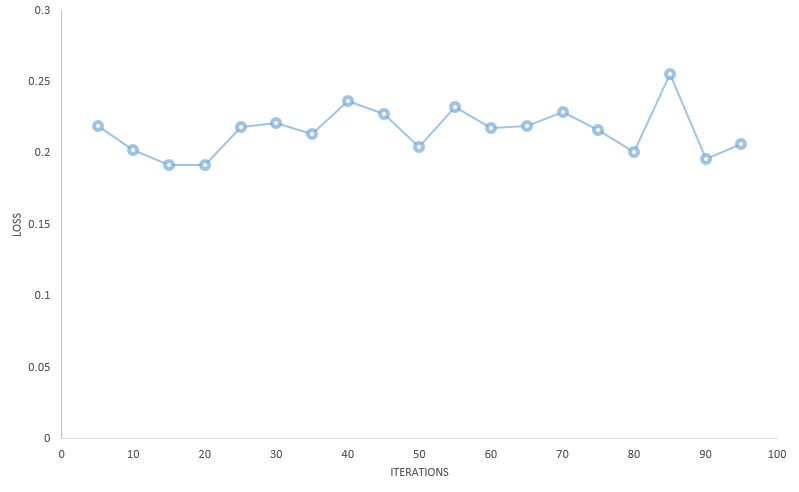
\includegraphics[height = 4cm, width=6cm]{report/perceptronx.png} \\
(fig:F2)
\end{center}
\begin{center}
SVM: \\  
\vspace{0.06cm} 
\begin{tabular}{|l|l|l|}
\hline
Kernel                                                           & Accuracy & Macro Avg. \\ \hline
Linear                                                           & 0.8394    & 0.842      \\ \hline
\begin{tabular}[c]{@{}l@{}}rbf \end{tabular} & 0.7867   & 0.7855
\\ \hline
\begin{tabular}[c]{@{}l@{}}Polynomial\\ (degree= 2)\end{tabular} & 0.6201   & 0.7542     \\ \hline
\begin{tabular}[c]{@{}l@{}}Polynomial\\ (Degree= 4)\end{tabular} & 0.31     & 0.77       \\ \hline
\end{tabular}
\end{center}
\vspace{0.04cm} 

\noindent{Logistic Regression: \\
    Learning rate = 0.012, Iterations =100,000 \\
    lambda = 0.0001  Accuracy = 0.778 
    
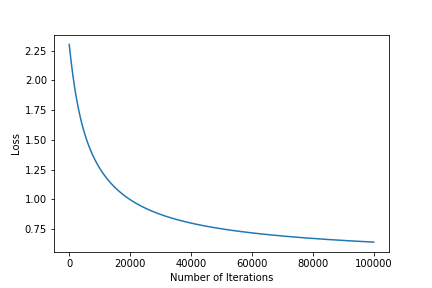
\includegraphics[height = 4cm, width=8cm]{report/svm_100k.png}
}


\subsection{Conclusion}
\noindent  The perceptron algorithm could not converge. Error curve on training set (fig:F2) shows the non-monotonic behavior of model indicating that the data is not linearly separable. The best accuracy 0.839 was obtained in case of SVM with linear kernel. Logistic regressions seems to work best when we have regularisation parameter lambda close to zero. The loss curve seems to saturate after 100k iterations. FLDA best accuracy was found to be 0.79 when we retained large number of components (300) after PCA.

\subsection{References}

\noindent [1] Fashion MNIST Reader. Retrieved from https://github.com/zalandoresearch/fashion-mnist/blob/master/utils/mnist\_reader.py\\
\noindent [2] Metric for multiclass classification. Retrieved from https://stats.stackexchange.com
/questions/51296/

\end{document}


